\documentclass[letterpaper,9pt,twocolumn,twoside,]{pinp}

%% Some pieces required from the pandoc template
\providecommand{\tightlist}{%
  \setlength{\itemsep}{0pt}\setlength{\parskip}{0pt}}

% Use the lineno option to display guide line numbers if required.
% Note that the use of elements such as single-column equations
% may affect the guide line number alignment.

\usepackage[T1]{fontenc}
\usepackage[utf8]{inputenc}

% pinp change: the geometry package layout settings need to be set here, not in pinp.cls
\geometry{layoutsize={0.95588\paperwidth,0.98864\paperheight},%
  layouthoffset=0.02206\paperwidth, layoutvoffset=0.00568\paperheight}

\definecolor{pinpblue}{HTML}{185FAF}  % imagecolorpicker on blue for new R logo
\definecolor{pnasbluetext}{RGB}{101,0,0} %



\title{House Prices In New York}

\author[]{Ishaan Singh}


\setcounter{secnumdepth}{0}

% Please give the surname of the lead author for the running footer
\leadauthor{}

% Keywords are not mandatory, but authors are strongly encouraged to provide them. If provided, please include two to five keywords, separated by the pipe symbol, e.g:
 

\begin{abstract}
This project aims to investigate the various features of properties in
the Saratoga County in New York State that affect its price, by creating
a multiple linear regression model which should ideally work well with
other random samples of data too. Through our model selection process,
the variables that are determined to have significant explanatory power
to explain the variation in house prices are: the lot size, whether it
is waterfront property, the number of rooms, bedrooms and bathrooms, the
living area, the type of heating system, whether it is a new
construction, whether it contains central air conditioning, and the land
value. This forms our restricted model that shall be used for
predictions. The testing of the model against the unrestricted full
model indicates a similar fit with respect to R-squared and adjusted
R-squared values, similar RMSE and MAE errors, and a better AIC and BIC
fit for our chosen restricted model when compared to the unrestricted
model. Hence, the variables we select in our final restricted model can
indeed be confirmed to be significant in their explanatory power for
predicting house prices, but this is limited to data from 2006 and
without other important attributes such as geographic location, suburb
data, parking spaces, proximity to other amenities etc. we cannot claim
to have a perfect model.
\end{abstract}

\dates{This version was compiled on \today} 


% initially we use doi so keep for backwards compatibility
% new name is doi_footer


\begin{document}

% Optional adjustment to line up main text (after abstract) of first page with line numbers, when using both lineno and twocolumn options.
% You should only change this length when you've finalised the article contents.
\verticaladjustment{-2pt}

\maketitle
\thispagestyle{firststyle}
\ifthenelse{\boolean{shortarticle}}{\ifthenelse{\boolean{singlecolumn}}{\abscontentformatted}{\abscontent}}{}

% If your first paragraph (i.e. with the \dropcap) contains a list environment (quote, quotation, theorem, definition, enumerate, itemize...), the line after the list may have some extra indentation. If this is the case, add \parshape=0 to the end of the list environment.


\hypertarget{introduction}{%
\subsection{\texorpdfstring{\textbf{Introduction}}{Introduction}}\label{introduction}}

The aim of this investigation is to create a multiple regression model
to allow us to predict house and property prices in New York state, and
not just specific counties or neighbourhoods. The goal is to make a
model consisting of attributes that significantly influence pricing
while also looking to avoid over-fitting. Doing so, shall require the
dropping of variables and attributes that do not improve the fit and
performance of the model, while also being aware of the fact that there
are attributes and features of properties that are not a part of this
data set, but which may provide significantly more explanatory power
than the attributes that are dropped from the model.

\hypertarget{data-description}{%
\subsection{\texorpdfstring{\textbf{Data
Description}}{Data Description}}\label{data-description}}

This
\href{https://dasl.datadescription.com/datafile/housing-prices-ge19}{data
set} contains observations for 1734 houses and properties. It is a
random sample that has been gathered from
\href{https://rdrr.io/cran/mosaicData/man/SaratogaHouses.html}{housing
price data for the Saratoga County} in New York State in 2006. The data
types of the information in this file include both Qualitative and
Quantitative. A quick examination of the data set through the creation
of boxplots did not indicate any concerning characteristics among any
variables. The categorical variables in the data were converted into
\emph{factor} types. This is a cross-sectional data set which contains
the following attributes: + prices (USD); + size of the lot (acres); +
age of the house (years); + land value (USD); + living area (square
feet); + percentage of neighbourhood that has graduated from college
(\%); + number of bedrooms; + number of fireplaces; + bathrooms, rooms;
+ type of heating system and the fuel used for it; + the type of sewer
system; + whether the property includes a waterfront; + whether it's a
new construction; + whether the house has central air conditioning.

\hypertarget{analysis-and-model-selection}{%
\subsection{\texorpdfstring{\textbf{Analysis and Model
Selection}}{Analysis and Model Selection}}\label{analysis-and-model-selection}}

The simplest model to select would be the unrestricted model that
contains every single attribute from the data set. However, simply
picking an unrestricted data set could result in the addition of
variables that do not contribute to predicting house prices in any
meaningful way. Additionally, we get rid of the \emph{Test} attribute
from both models. This attribute is not an explanatory variable, but is
instead a binary variable used to create a 75-25 training and testing
data split. However, since we shall implement \emph{k}-fold
cross-validation, this attribute is not of any use to us.

\begin{ShadedResult}
\begin{verbatim}
#                          Estimate   Std. Error
#  (Intercept)         2.697224e+03 6.233207e+03
#  Lot.Size            7.527732e+03 2.041817e+03
#  Waterfront          1.195883e+05 1.532911e+04
#  Land.Value          9.074394e-01 4.591304e-02
#  New.Construct      -4.179808e+04 7.055142e+03
#  Central.Air         1.078712e+04 3.361776e+03
#  Heat.TypeHot Air    8.617811e+03 3.999565e+03
#  Heat.TypeHot Water -4.058083e+03 5.000203e+03
#  Heat.TypeNone      -4.750198e+04 2.403641e+04
#  Living.Area         6.999255e+01 4.495365e+00
#  Bedrooms           -8.554149e+03 2.530940e+03
#  Bathrooms           2.572424e+04 3.140393e+03
#  Rooms               3.051788e+03 9.596958e+02
\end{verbatim}
\end{ShadedResult}

The method used to test the significance of was an F-test of the terms.
Any variables with coefficient estimates that had a p-value greater than
1\%, were removed from the model, which is the chosen level of
significance. The tests were repeated and variables were deleted from
the model as and when they proved to have an insignificant effect on the
regressand. The results of our testing lead us to drop the \emph{sewer
type}, \emph{number of fireplaces}, \emph{type of fuel} for the heating
system and the \emph{age} of the property as regressors for our new
model. The only surprising omission from the model is the \emph{age} of
the property, however, this too has an explanation. Given that the model
also has a binary variable to indicate whether a property is ``new''
(even though the criteria for being new isn't specified), it may capture
most of the effect that a house being newer has on the price, leaving
the \emph{age} attribute to explain much less of the variation in
prices. The key insight from this process is that the removal of an
attribute does not mean that we may conclude that the respective
attribute has no explanatory power, but rather, that it does not explain
the variation in the price any more than the existing variables in the
model, at the chosen level of significance.

Hence, we may now interpret the coefficients. For example, an additional
acre of lot size in a property is associated with an increase in the
total price by approximately USD 7528; all other variables held
constant. Similarly, if we examine a categorical variable such as
whether or not the property has central air conditioning, we see that
properties that have it have an associated higher price by approximately
USD 10787. All the coefficients obtained through the regression indicate
a relationship in the expected direction, except for the number of
Bedrooms and whether the property is a new construction. In the case of
the number of bedrooms, this may be due to the presence of other
variables such as Bathrooms, Rooms, and Living Area, which may capture
those effects. New constructions may cause uncertainty in the minds of
consumers regarding the quality and durability of houses, hence newer
constructions may have a negative relationship with prices.

From our results, the elimination of insignificant regressors reduced
the R-squared value very minutely, which would be expected. However, the
\textbf{adjusted} R-squared value increases very slightly for our
restricted model, thus indicating a model with a fit that is at least as
good as the full model, if not very slightly better. We would also
expect new model to be less prone to over-fitting, due to the omission
of regressors that may not improve fit for any other sample.

\hypertarget{assumption-checking}{%
\subsection{\texorpdfstring{\textbf{Assumption
Checking}}{Assumption Checking}}\label{assumption-checking}}

Now that an appropriate model has been selected, we may wish to test its
performance. However, before doing so we must ensure that the selected
models satisfies some key assumptions of Ordinary Least Squares
regression. The assumptions that are tested include:

\begin{enumerate}
\def\labelenumi{\arabic{enumi}.}
\tightlist
\item
  \textbf{Linearity}. This assumption can be tested by regressing the
  \emph{price} against all the remaining numeric regressors (See
  Appendix 1). In order for the linearity assumption to be satisfied,
  the plots should indicate a roughly linear relationship between the
  \emph{price} and the regressor. The plots do in fact indicate that
  this assumption is satisfied, and hence, no additional variables need
  to be dropped or transformed.
\item
  \textbf{Conditional Mean Independence}. In order to satisfy this
  assumption, the expected value of error should be zero conditional on
  all regressors (See Appendix 1, top left chart). This is expected to
  be the case since the data is cross-sectional and not a time series.
  Observing the plot for the residuals against the indices displays no
  obvious positive or negative trend, with the mean value of the
  residuals around 0. Hence, this assumption is also satisfied.
\item
  \textbf{Homoskedasticity}. For the errors to be homoskedastic, it is
  required the variance of the errors are constant when conditional on
  the regressors. This assumption is tested by observing the plots of
  the residuals against the various regressors (See Appendix 2). From
  the plots we do not detect any strong evidence of heteroskedasticity
  and hence, this assumption is satisfied.
\item
  \textbf{Normality of Errors}. We test this assumptions by observing
  the distribution of the residuals using a QQ-plot. Doing so shows that
  the residuals are largely normally distributed. Given that the sample
  size we are dealing with is large, we can rely on the Central Limit
  Theorem and the evidence from the plot to satisfy this assumption.
\item
  \textbf{No Perfect Collinearity}. Since our model consists of multiple
  regressors, it is important that there doesn't exist any perfect
  correlation between the regressors. This assumption is tested by the
  inspection of a correlation matrix. Doing so does not reveal any
  ``perfect'' correlation, despite some strong correlation between
  regressors such as the \emph{living area} and \emph{rooms}. Hence,
  this result does not warrant the deletion of any regressors, which
  allows us to satisfy this assumption.
\end{enumerate}

By satisfying all the assumptions described above, we get two important
results: 1. The model being estimated is \textbf{valid}; 2. The
coefficient estimates we obtain are going to be the \textbf{Best Linear
Unbiased Estimators}. Before proceeding we also tested the same
assumptions for the full unrestricted model so as to ensure that the
later stage performance testing and comparisons were valid. The full
model also satisfies the relevant assumptions.

\hypertarget{results}{%
\subsection{\texorpdfstring{\textbf{Results}}{Results}}\label{results}}

We train and test our model using 17-fold cross-validation. This is
alternative to simply performing basic residual evaluations and arriving
at conclusions using R-squared values etc. Using cross-validation allows
us to get some indication of how well the chosen model is likely to
perform when it is provided data that has not already been used for
training the model. Since the method selected has 17 folds, it helps us
reduce the overall variance of resulting estimate. At the same time,
subset of the data contains 102 observations which is also large enough
to help reduce bias. Hence, the 17-fold cross-validation helps provide
an appropriate bias-variance trade-off. This training process is done
for both the chosen restricted model and the full unrestricted model, in
order to make comparisons.

After completing the cross-validation process we can compare the Root
Mean Squared Errors and Mean Absolute Errors for the full model and the
our chosen restricted model (See Appendix 3). This comparison reveals
that while the full unrestricted model has overall smaller errors in
comparison to the restricted model, the difference is minuscule.

For a test of our models predictions we can generate a prediction and
confidence interval. This is done by picking a random observation from
the data set with a price of USD 140000. Our model makes a prediction of
USD 161302.25. The 99\% prediction interval generated equals
{[}10714.61, 311889.9{]}, while the 99\% confidence interval is
{[}149200.4, 173404{]}. The prediction interval captures the actual
price of the property too and is wider than the confidence interval,
which is to be expected.

Another set of metrics that we shall use to compare our chosen
restricted model and the unrestricted full model is AIC and BIC. The
\textbf{Akaike Information Criterion} estimates the relative distance
between the true likelihood function of the data and the fitted
likelihood function of the model. The \textbf{Bayesian Information
Criterion} estimates the function of the posterior probability of a
model being true, using Bayesian analysis. In both instances, a lower
value tends to indicate a better fit.

After calculating the AIC and BIC for the restricted and unrestricted
model, we find that our chosen model has a lower AIC and BIC by 12 and
66 values approximately, which is a significant difference that favours
our chosen model over the full unrestricted one.

\hypertarget{discussion-and-conclusion}{%
\subsection{\texorpdfstring{\textbf{Discussion and
Conclusion}}{Discussion and Conclusion}}\label{discussion-and-conclusion}}

Some limitations that could be addressed in future are:

\begin{enumerate}
\def\labelenumi{\arabic{enumi}.}
\tightlist
\item
  Accessing the geographic locations or suburbs in which each property
  is located in order to create a more thorough model.
\item
  Having data for other attributes such as the proximity to schools and
  other amenities, parking spaces etc will assist testing a more diverse
  range of variables which could affect house prices.
\item
  Using data from throughout New York State, to build a model that is
  useful in predicting the property prices throughout the state.
\item
  The current model should not be used to predict current house prices.
  Since our model has been trained using cross-sectional data from 2006,
  it does not allow for trend or seasonal corrections.
\end{enumerate}

In conclusion, after observing the slightly increased adjusted R-squared
value, only a slightly larger RMSE and MAE value for the new restricted
model, and the lower AIC and BIC values we can be reasonably confident
that our chosen restricted model of Price \textasciitilde{} Lot.Size +
Waterfront + Land.Value + New.Construct + Central.Air + Heat.Type +
Living.Area + Bedrooms + Bathrooms + Rooms is a better choice and
reduces the risk of over-fitting.

\hypertarget{references}{%
\subsection{\texorpdfstring{\textbf{References}}{References}}\label{references}}

\begin{enumerate}
\def\labelenumi{\arabic{enumi}.}
\tightlist
\item
  Wickham et al., (2019). Welcome to the tidyverse. Journal of Open
  Source Software, 4(43), 1686,
  \url{https://doi.org/10.21105/joss.01686}
\item
  Karl W Broman (2015), R/qtlcharts: interactive graphics for
  quantitative trait locus mapping.
  \url{https://pubmed.ncbi.nlm.nih.gov/25527287/}
\end{enumerate}

\hypertarget{appendix-1-linearity-and-independence-assumption-testing}{%
\subsection{\texorpdfstring{\textbf{Appendix 1: Linearity and
Independence Assumption
Testing}}{Appendix 1: Linearity and Independence Assumption Testing}}\label{appendix-1-linearity-and-independence-assumption-testing}}

\begin{center}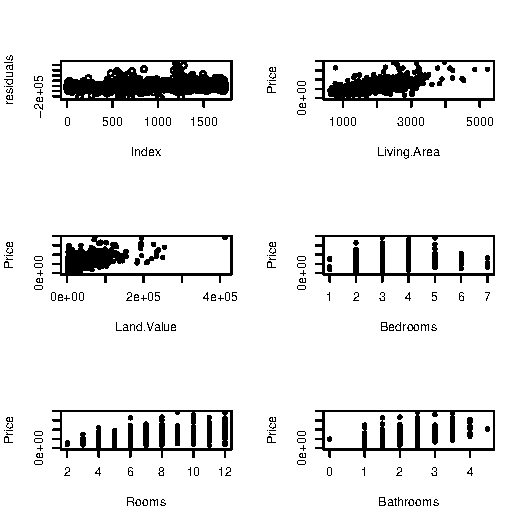
\includegraphics{Report_files/figure-latex/unnamed-chunk-4-1} \end{center}

\hypertarget{appendix-2-homoskedasticity-assumption-testing}{%
\subsection{\texorpdfstring{\textbf{Appendix 2: Homoskedasticity
Assumption
Testing}}{Appendix 2: Homoskedasticity Assumption Testing}}\label{appendix-2-homoskedasticity-assumption-testing}}

\begin{center}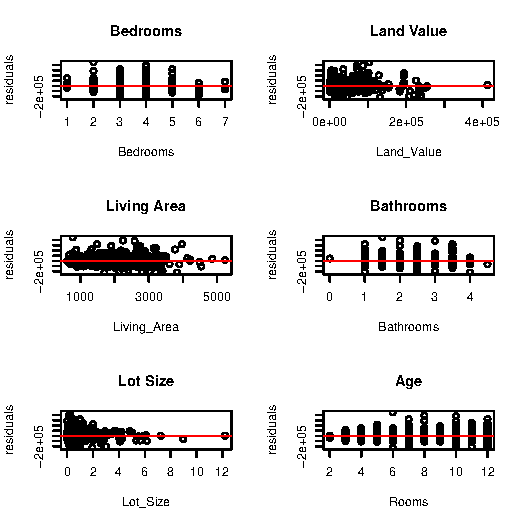
\includegraphics{Report_files/figure-latex/unnamed-chunk-5-1} \end{center}

\hypertarget{appendix-3-rmse-and-mae-boxplots}{%
\subsection{\texorpdfstring{\textbf{Appendix 3: RMSE and MAE
Boxplots}}{Appendix 3: RMSE and MAE Boxplots}}\label{appendix-3-rmse-and-mae-boxplots}}

\begin{center}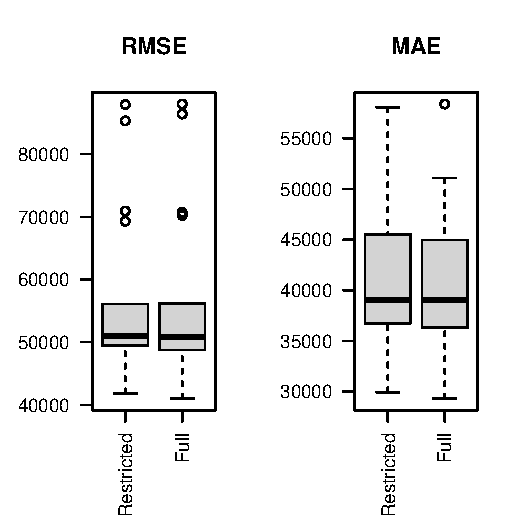
\includegraphics{Report_files/figure-latex/unnamed-chunk-6-1} \end{center}

\hypertarget{appendix-4-final-model-equation}{%
\subsection{\texorpdfstring{\textbf{Appendix 4: Final Model
Equation}}{Appendix 4: Final Model Equation}}\label{appendix-4-final-model-equation}}

The final model is : Price \textasciitilde{} Lot.Size + Waterfront +
Land.Value + New.Construct + Central.Air + Heat.Type + Living.Area +
Bedrooms + Bathrooms + Rooms

So using the table below, having a waterfront will increase the value by
111958.83 Dollars.

\begin{ShadedResult}
\begin{verbatim}
#                          Estimate   Std. Error
#  (Intercept)         2.697224e+03 6.233207e+03
#  Lot.Size            7.527732e+03 2.041817e+03
#  Waterfront          1.195883e+05 1.532911e+04
#  Land.Value          9.074394e-01 4.591304e-02
#  New.Construct      -4.179808e+04 7.055142e+03
#  Central.Air         1.078712e+04 3.361776e+03
#  Heat.TypeHot Air    8.617811e+03 3.999565e+03
#  Heat.TypeHot Water -4.058083e+03 5.000203e+03
#  Heat.TypeNone      -4.750198e+04 2.403641e+04
#  Living.Area         6.999255e+01 4.495365e+00
#  Bedrooms           -8.554149e+03 2.530940e+03
#  Bathrooms           2.572424e+04 3.140393e+03
#  Rooms               3.051788e+03 9.596958e+02
\end{verbatim}
\end{ShadedResult}

%\showmatmethods





\end{document}

